\section{Design of FFT architecture via folding transformation}
\subsection{Parallel radix-$2^3$ 16-Points}
\begin{frame}
  \frametitle{\textbf{Table of Contents}}
  \begin{center}
    {\vspace{-1.5cm}\Large \textbf{Section \thesection}\vspace{0.5cm}}
    \begin{beamercolorbox}[
      sep=8pt,center]{part title}
      \usebeamerfont{part title}
      \textbf{\insertsection}
    \end{beamercolorbox}
  \end{center}
\end{frame}


\begin{frame}
	\frametitle{\textbf{Design of FFT architecture via folding transformation}}
	\framesubtitle{\secname : \subsecname}
	
	\begin{block}{\centering \textbf{Folding Set}}
		\begin{itemize}\justifying\footnotesize
        	\item Is an ordered set of operations executed by the same functional unit.
        	\item Each folding set contains K entries, where K is called the folding factor.
        	\item The operation in the \textit{j}th position (where goes from 0 to K-1) is called the folding order.
       	\end{itemize}
	\end{block}

	\begin{block}{\centering \textbf{Folding Equations}}
		\begin{itemize}\justifying\footnotesize
			\item Consider an edge $e$ connecting the nodes \textit{U} and \textit{V} with $w(e)$ delays. 
			\item The executions of the \textit{l}th iteration of \textit{U} and \textit{V} are scheduled at the time units $Kl+u$ and $Kl+v$ respectively, where $u$ and $v$ are the folding orders of the nodes \textit{U} and \textit{V}.
			\item  The folding equation for the edge $e$ is:
			\begin{equation}\label{eqn:fold_equation}
				D_F(U \to V) = Kw(e)-P_U+v-u
			\end{equation}
			where $P_U$ is the number of pipeline stages in the node \textit{U}.
	    \end{itemize}
	\end{block}
\end{frame}


\begin{frame}
	\frametitle{\textbf{Design of FFT architecture via folding transformation}}
	\framesubtitle{\secname : \subsecname}
		\vspace{-0.5cm}
	    \begin{columns}[t,onlytextwidth]
	      \begin{column}{0.45\linewidth}
			\begin{block}{\centering \textbf{Folding equations without retiming/pipeline}}	      	
	        	\begin{itemize} \justifying\footnotesize
					\item Consider the folding sets:  \vfill
					\scalebox{0.65}{
					\label{eq:foldingset_16}		 
		 			\parbox{\linewidth}{ 
					\begin{align*}
						A&= \{ A0,A2,A4,A6 \}  & A'&= \{ A1,A3,A5,A7 \} \\
						B&=\{ B1,B3,B0,B2 \}   &B'&=\{ B5,B7,B4,B6 \} 	\\
						C&=\{ C2,C1,C3,C0 \}   &C'&=\{ C6,C5,C7,C4 \} 	\\ 
						D&=\{ D3,D0,D2,D1 \}   &D'&=\{ D7,D4,D6,D5 \}  
					\end{align*}}}
				
					\item For example: \vfill
					\scalebox{0.8}{
		 			\parbox{\linewidth}{ 				
					\begin{align*}
						D_F(D3\to B3)&= v - u \\
								 &= 0 - 1 \\  
								 &= -1
					\end{align*}}}
					\item The folding equations can be derived for all edges. \vfill
	      		\end{itemize}
			\end{block}	      
	      \end{column}
	      \begin{column}{0.50\linewidth}
	      	      \vspace{1cm}
			    \begin{figure}[h!] \centering
	    			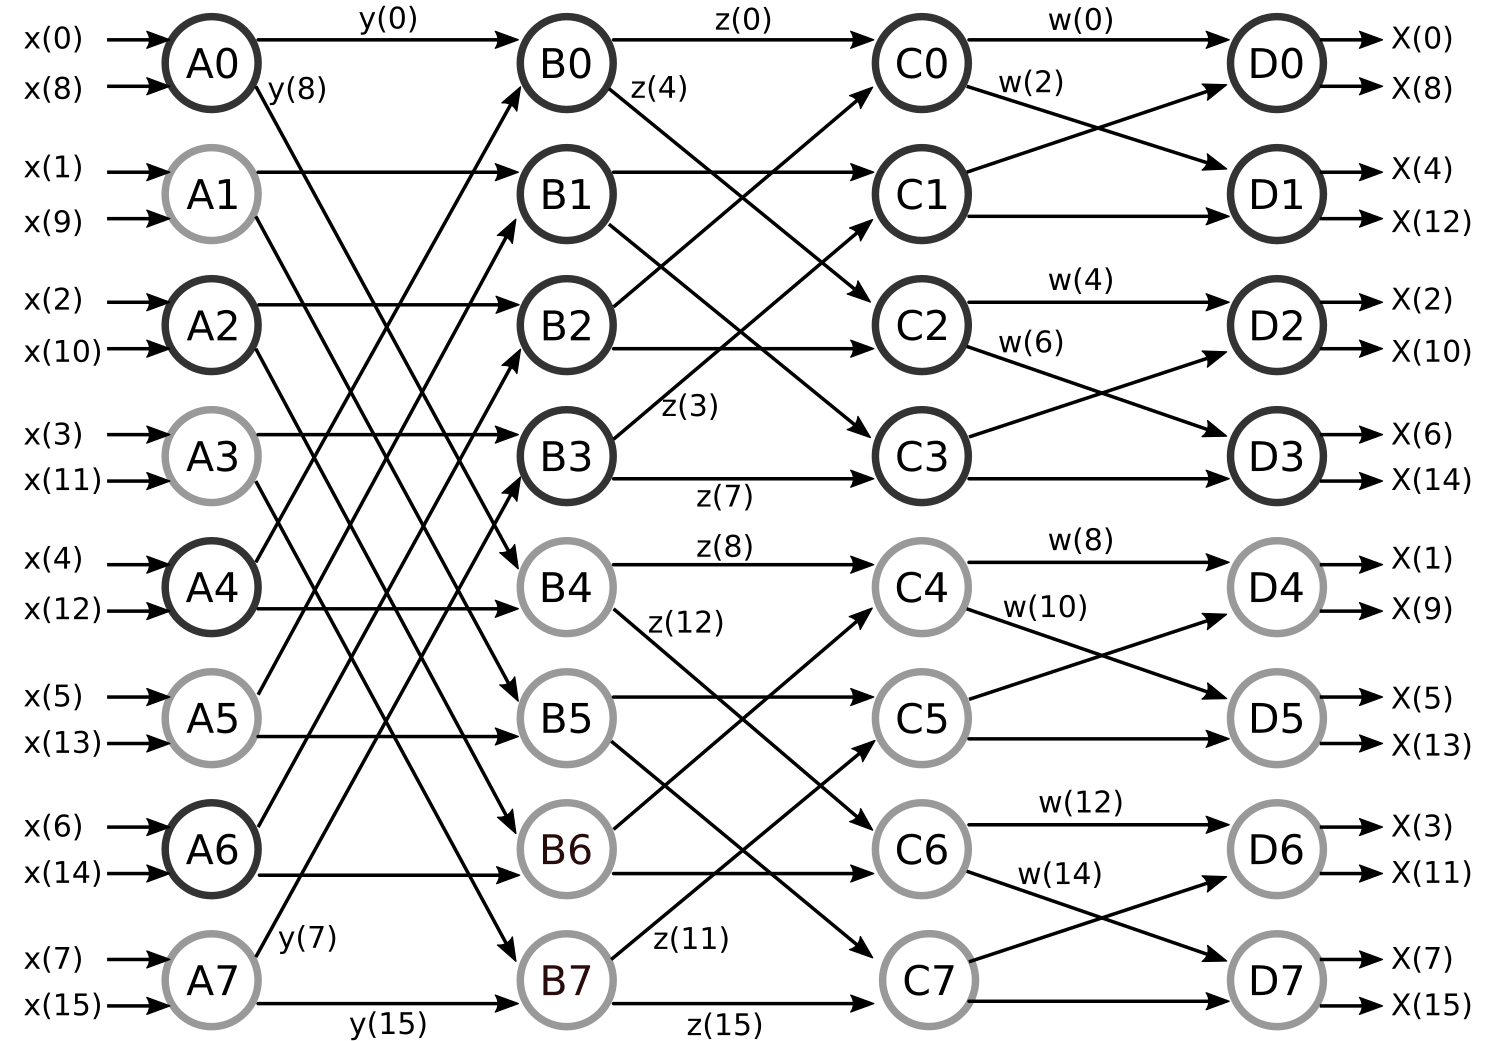
\includegraphics[width=0.45\paperwidth]{./image/16points_dfg.png}
	    			\caption{\footnotesize DFG of a radix-$2^3$ 16-point DIF DFT.}
	    		\end{figure}    
	      \end{column}
	    \end{columns}
\end{frame}




\begin{frame}
	\frametitle{\textbf{Design of FFT architecture via folding transformation}}
	\framesubtitle{\secname : \subsecname}
		\vspace{-0.5cm}
	    \begin{columns}[t,onlytextwidth]
	      \begin{column}{0.45\linewidth}
			\begin{block}{\centering \textbf{Folding equations with retimming/pipeline}}	      	
	        	\begin{itemize} \justifying\footnotesize
					\item For the folded system to be realizable, $D_F(U\to V)\geq0$ must hold for all the edges. \vfill
					\item For example: \vfill
						\scalebox{0.8}{
		 				\parbox{\linewidth}{ 				
						\begin{align*}
							D_F(D3\to B3)&= Kw(e) + v - u \\
								 &= 4(1) + 0 - 1 \\  
								 &= 3
						\end{align*}}}
						
					\item This result $D_F(U\to V)\geq0$ for all the edges.
					\item Applying the folding equations for all the edges, the number of registers required is 80. \vfill
	      		\end{itemize}
			\end{block}	      
	      \end{column}
	      \begin{column}{0.50\linewidth}
	      \vspace{1cm}
			    \begin{figure}[h!] \centering
	    			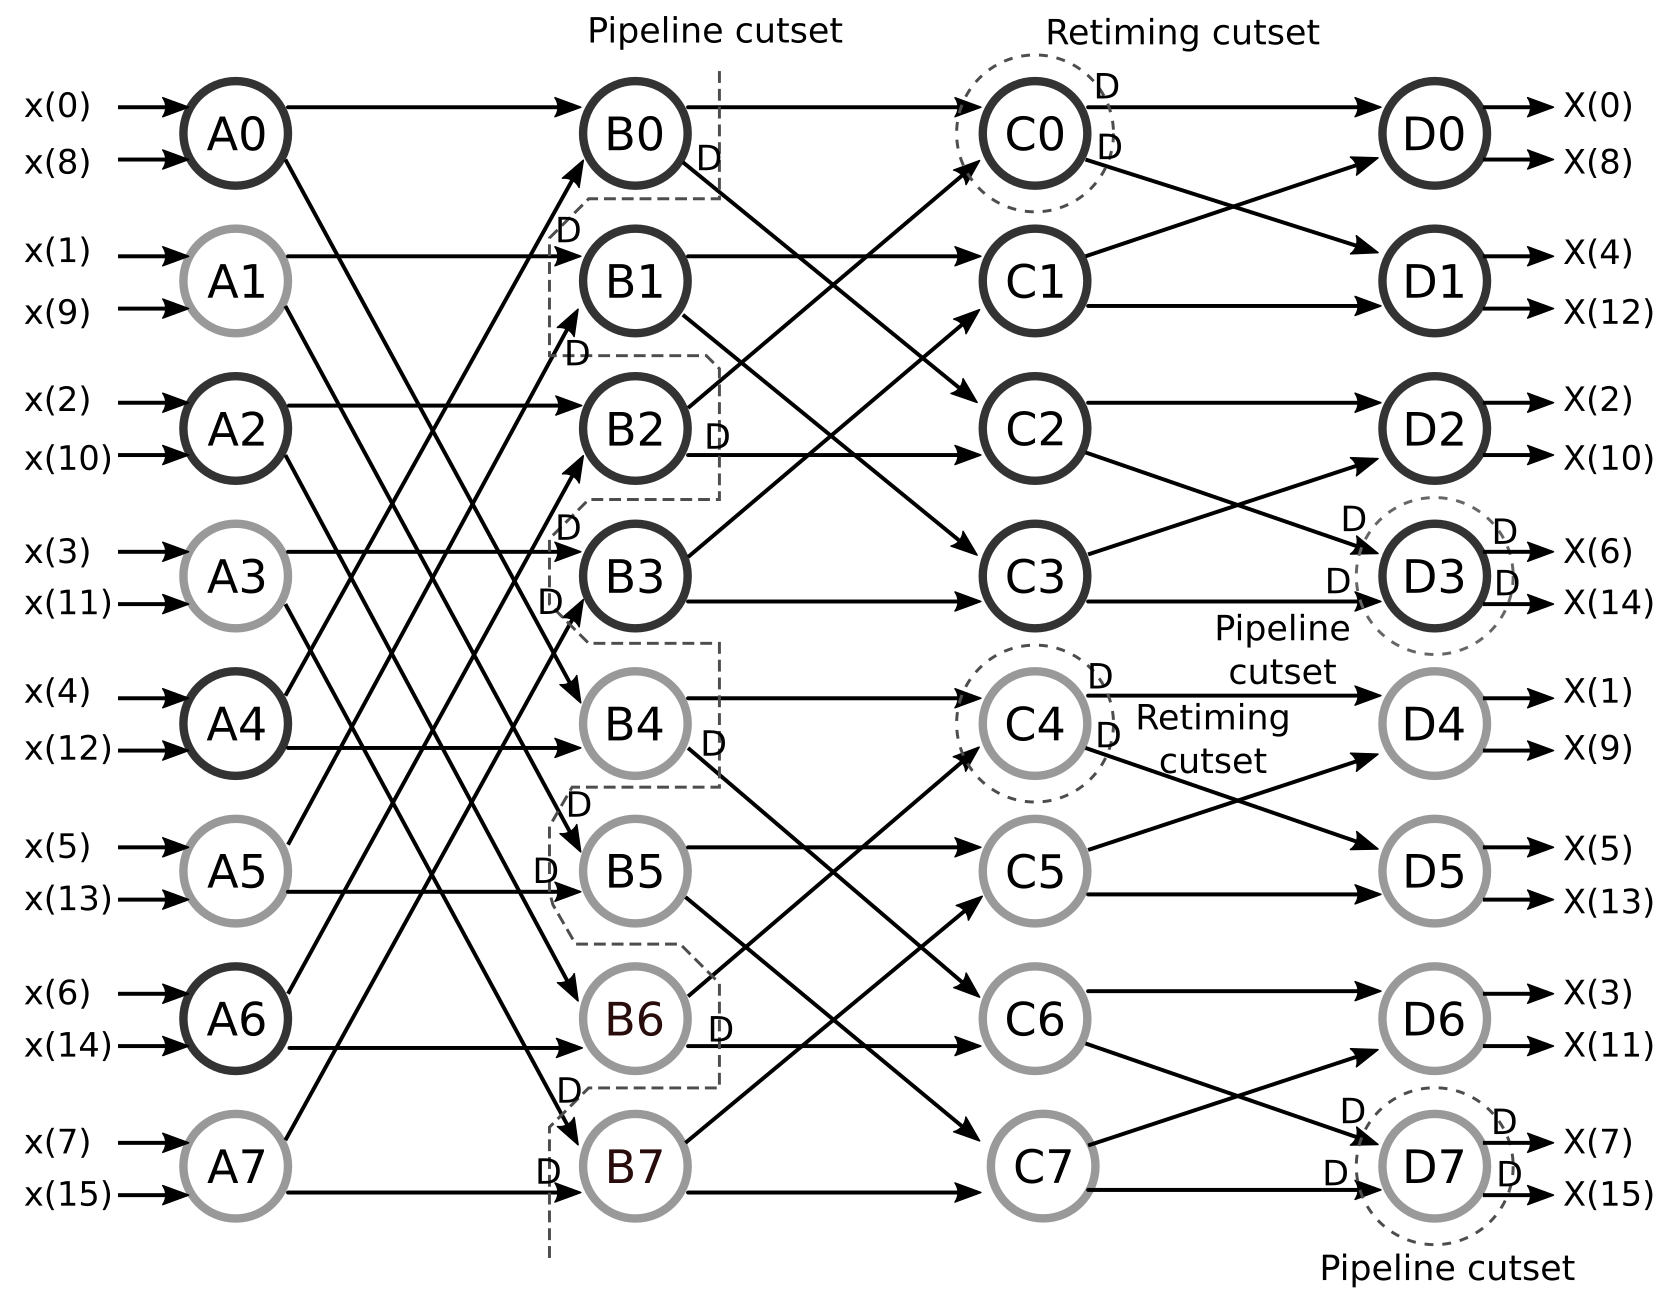
\includegraphics[width=0.45\paperwidth]{./image/16points_dfg_ret.png}
	    			\caption{\footnotesize DFG of a radix-$2^3$ 16-point DIF DFT applying pipeline and retiming.}
	    			\label{fig:16_point_ret}
	    		\end{figure}    
	      \end{column}
	    \end{columns}
\end{frame}

\begin{frame}
	\frametitle{\textbf{Design of FFT architecture via folding transformation}}
	\framesubtitle{\secname : \subsecname}
	\vspace{-0.5cm}
	 \begin{columns}[t,onlytextwidth]
	      \begin{column}{0.5\linewidth}
			\begin{block}{\centering \textbf{Lifetime analysis}}
				\begin{itemize}\justifying\footnotesize
					\item Is a procedure used to compute the minimun number of registers. \vfill
					\item For example, the variable $y_1$ be live during time units $n \in \{1,2,3,4\}$.
					\item The number of live variables $y_i$ during the time units $\{1,2,3,4,5\}$ is $\{4,8,8,8,4\}$. So the number of register for this stage is: \vfill
					\begin{equation*}
						max\{4,8,8,8,4\} = 8
					\end{equation*}
					\item The total number of registers is reduced from 80 to 20. \vfill
		       	\end{itemize}
			\end{block}
   		  \end{column}
   		  \begin{column}{0.5\linewidth}
   		  	 \vspace{-0.5cm}
   			\begin{figure}[h!] \centering
	    		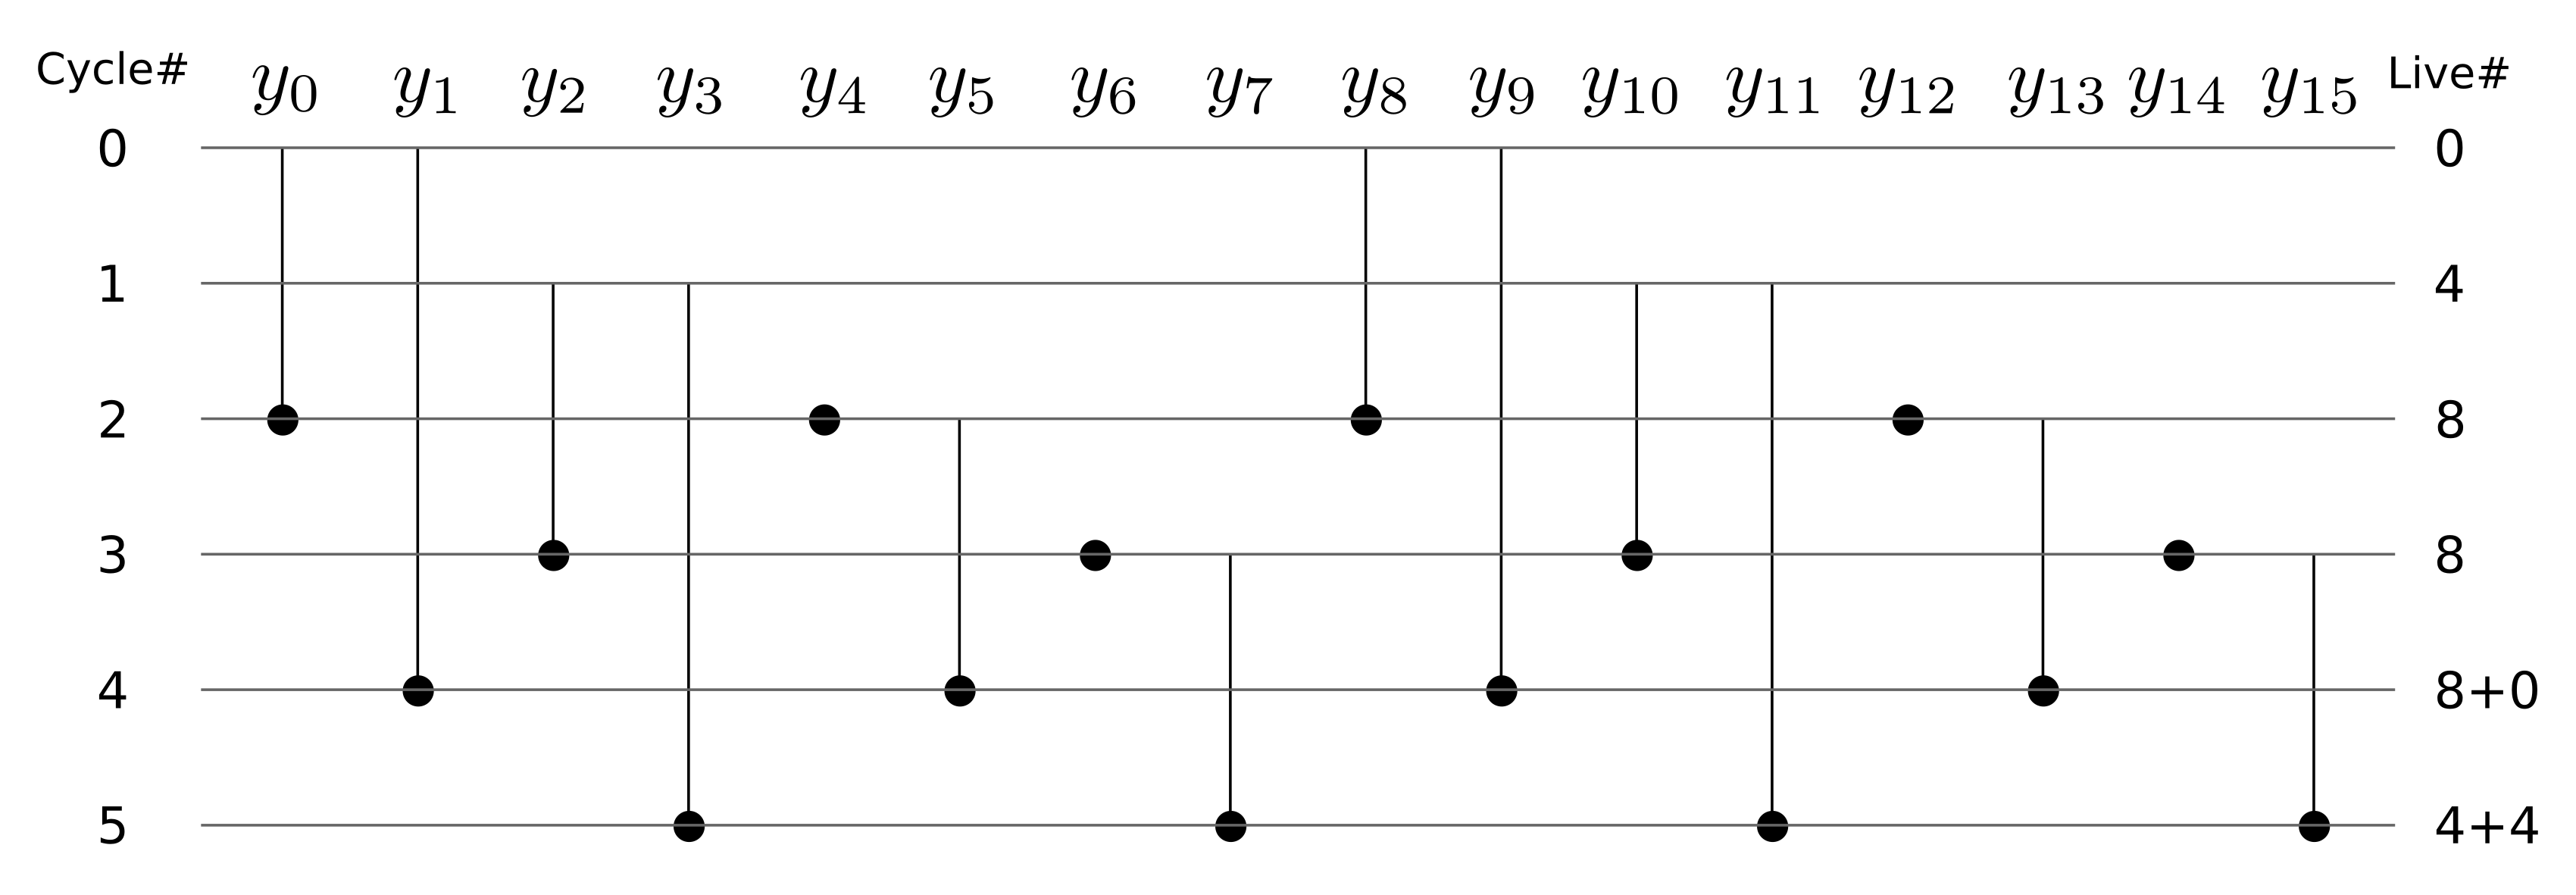
\includegraphics[width=0.40\paperwidth]{./image/life_chart_a.png}
	    		\caption{\footnotesize Lifetime chart for stage 1.}
	    	\end{figure}
	    	\vspace{-1cm}
	    	\begin{figure}[h!] \centering
	    		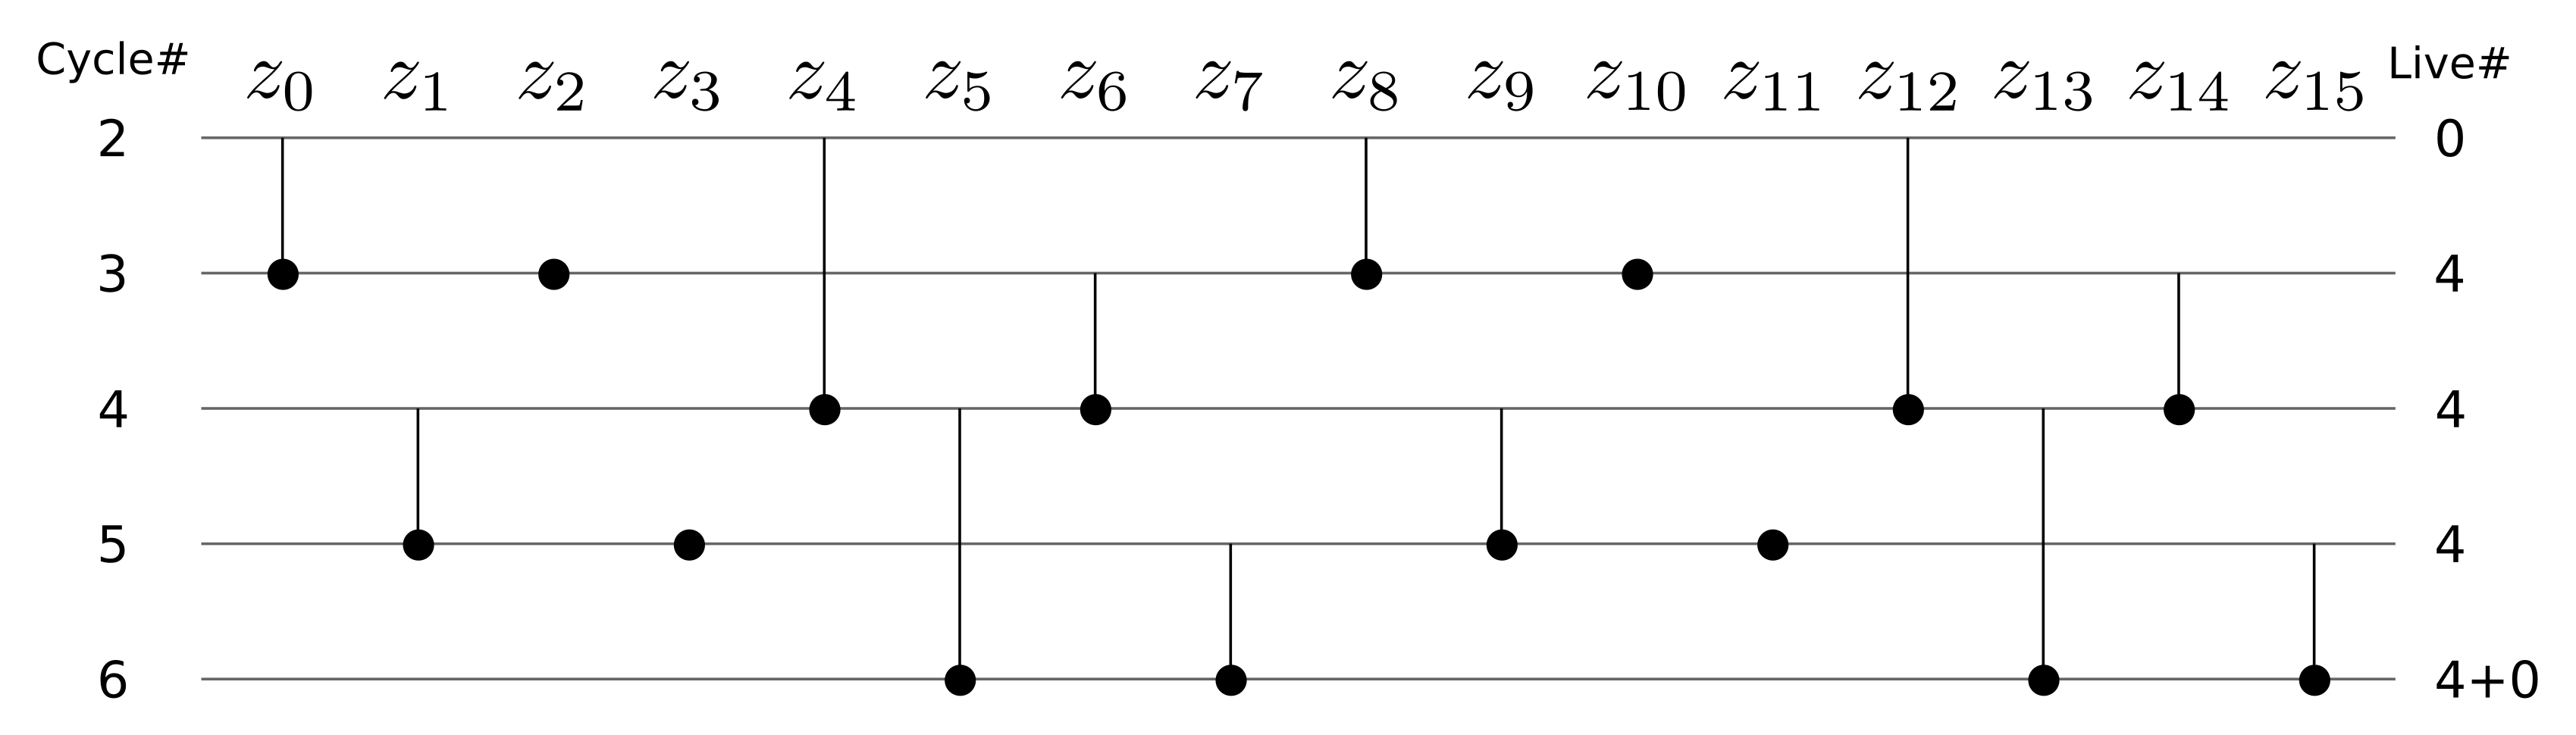
\includegraphics[width=0.40\paperwidth]{./image/life_chart_b.png}
	    		\caption{\footnotesize Lifetime chart for stage 2.}
	    	\end{figure}
			\vspace{-1cm}	    	
	    	\begin{figure}[h!] \centering
	    		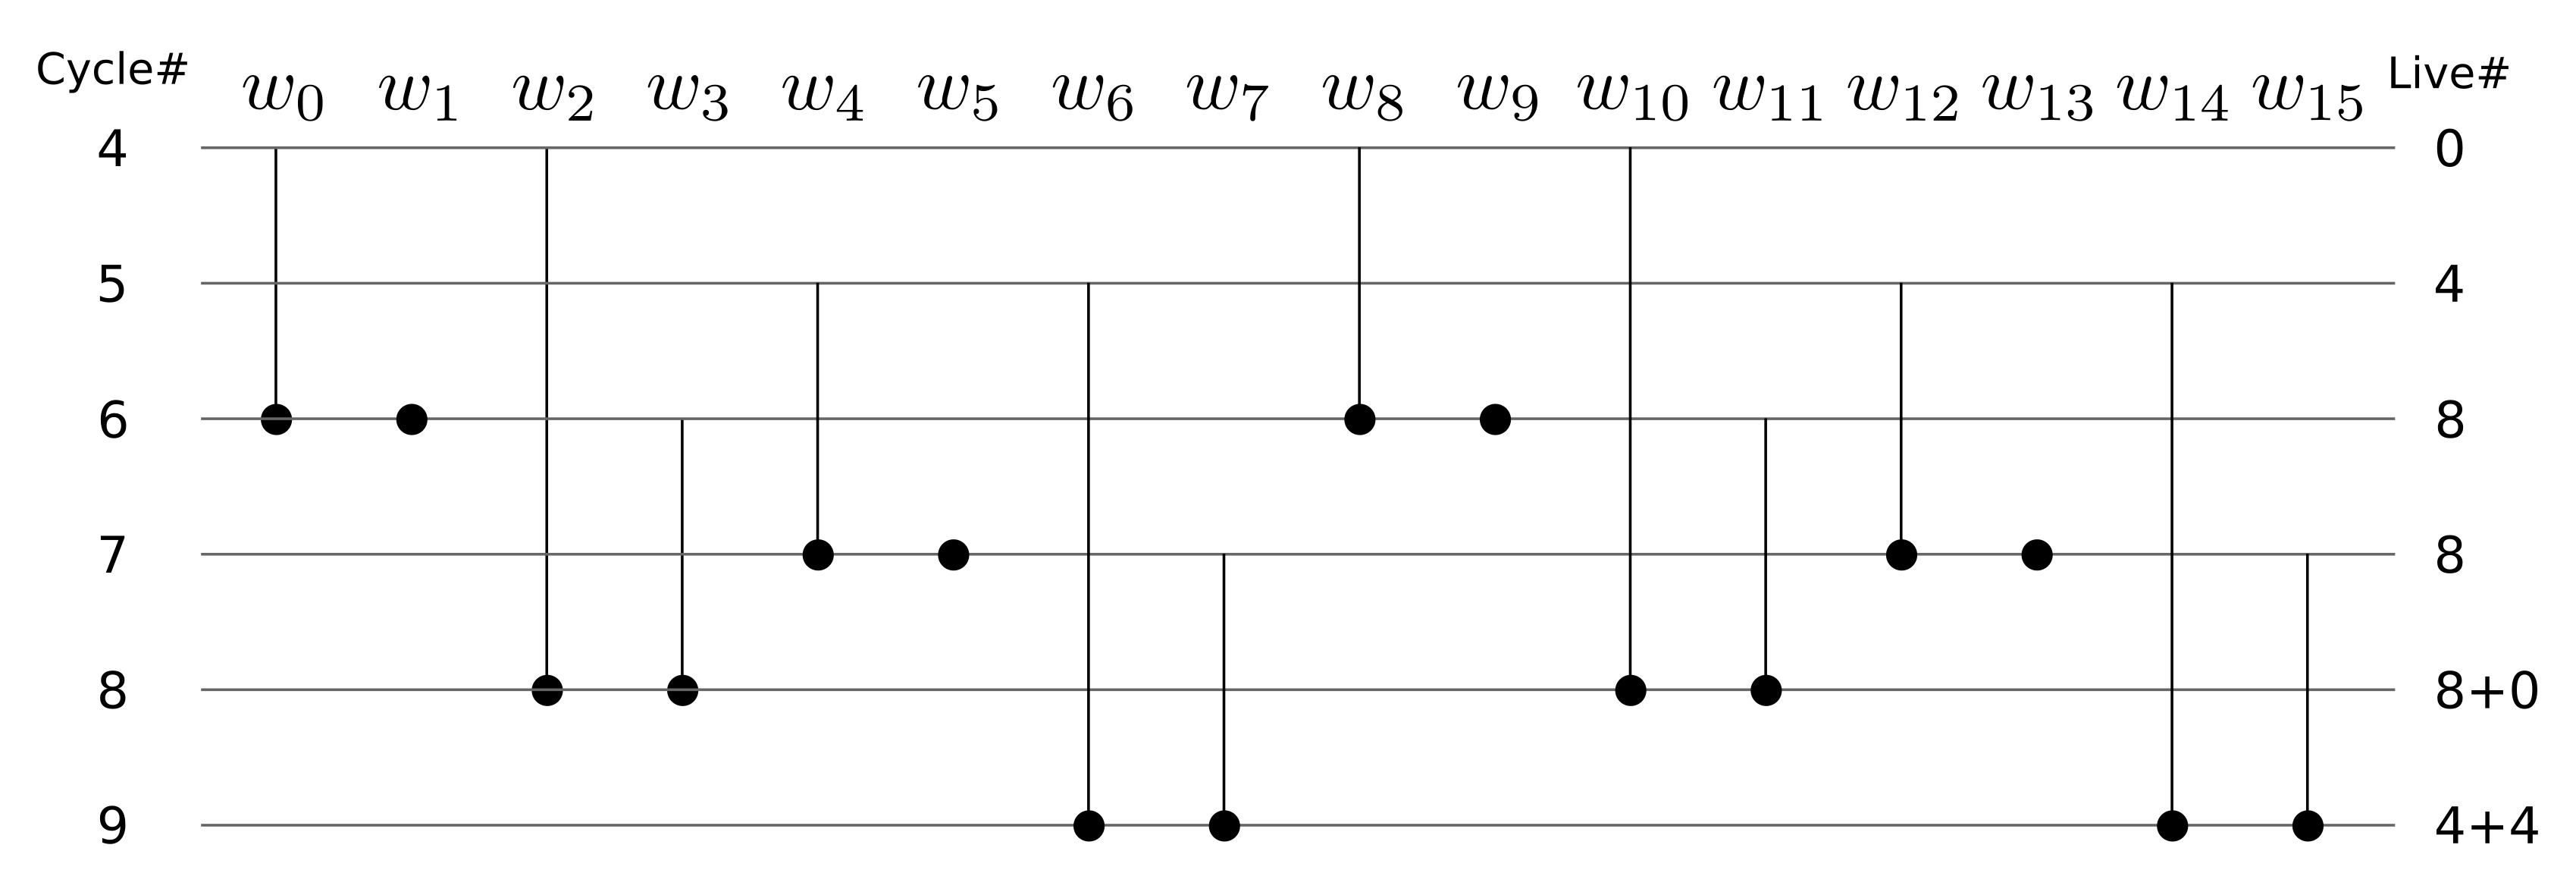
\includegraphics[width=0.40\paperwidth]{./image/life_chart_c.png}
	    		\caption{\footnotesize Lifetime chart for stage 3.}	    	
	    	\end{figure}  
   		\end{column}
	\end{columns}
\end{frame}

\begin{frame}
	\frametitle{\textbf{Design of FFT architecture via folding transformation}}
	\framesubtitle{\secname : \subsecname}
	\vspace{-0.5cm}
	 \begin{columns}[t,onlytextwidth]
	      \begin{column}{0.5\linewidth}
			\begin{block}{\centering \textbf{Forward Register Allcation}}
				\begin{itemize}\justifying\footnotesize
		        	\item This dictates how the variables are assigned to the minimum numbers of registers. \vfill
		        	\item If $R_i$ holds holds a variable in the current ctcle, then $R_{i+1}$ hold the same variable on the next cycle.
		       	\end{itemize}
			\end{block}
			\vspace{-0.3cm}
			\begin{figure}[h!] \centering
	    		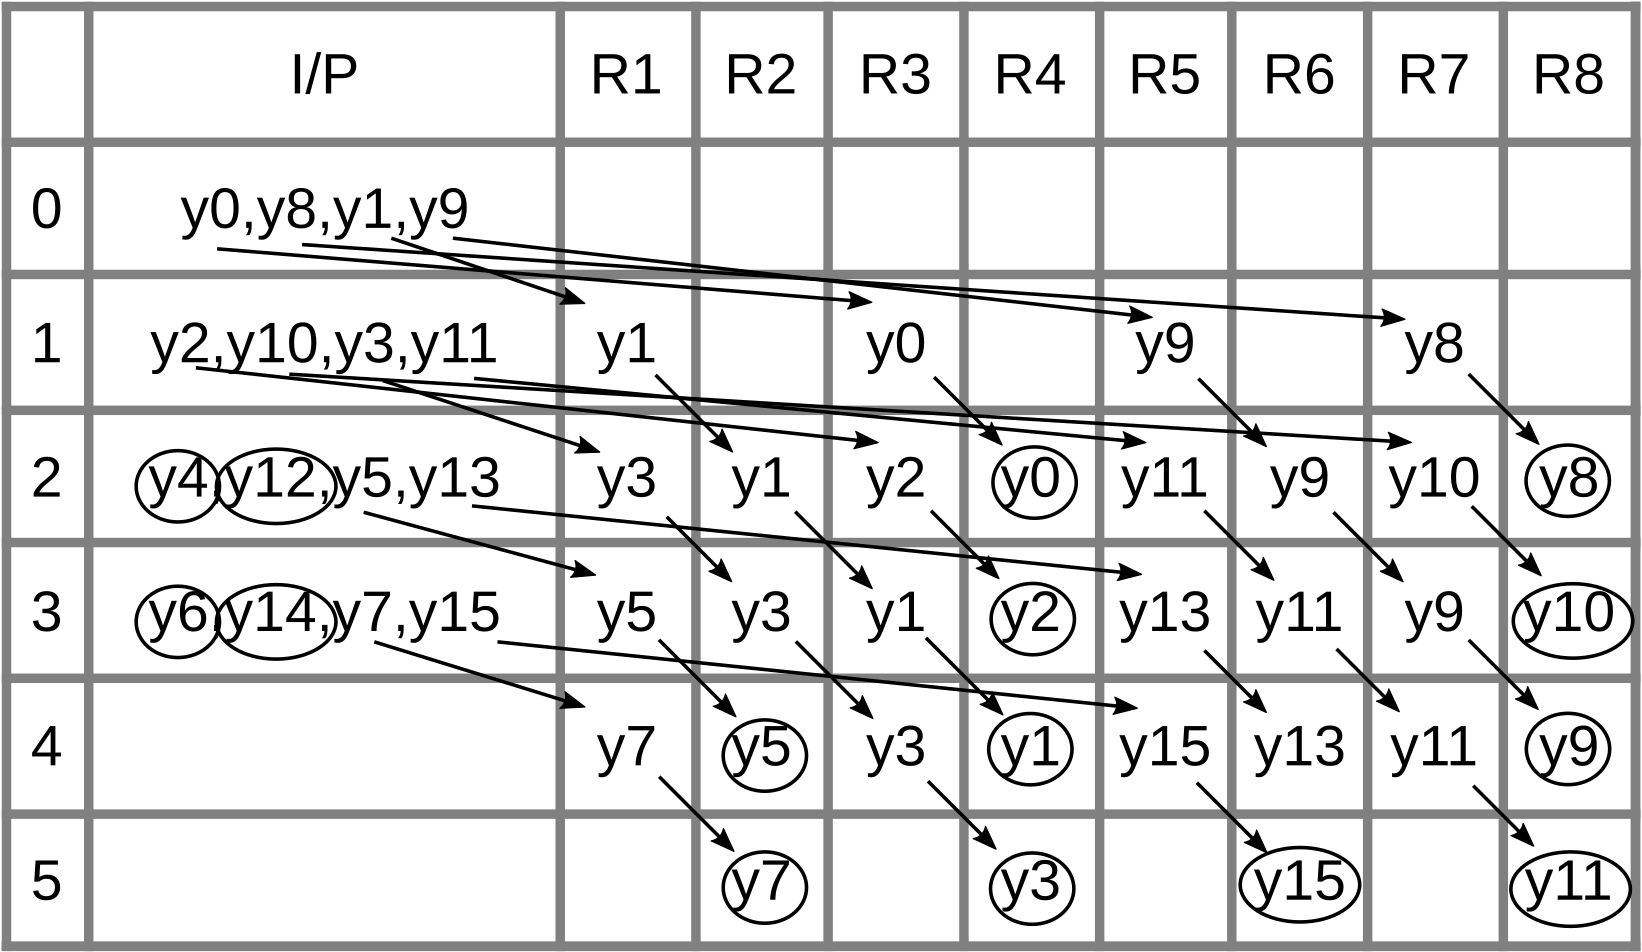
\includegraphics[height=0.30\paperheight]{./image/tab-life-a.png}
	    		\caption{\footnotesize Allocation table for stage 1.}
	    	\end{figure}
   		  \end{column}
   		  \begin{column}{0.45\linewidth}
   			\begin{figure}[h!] \centering
	    		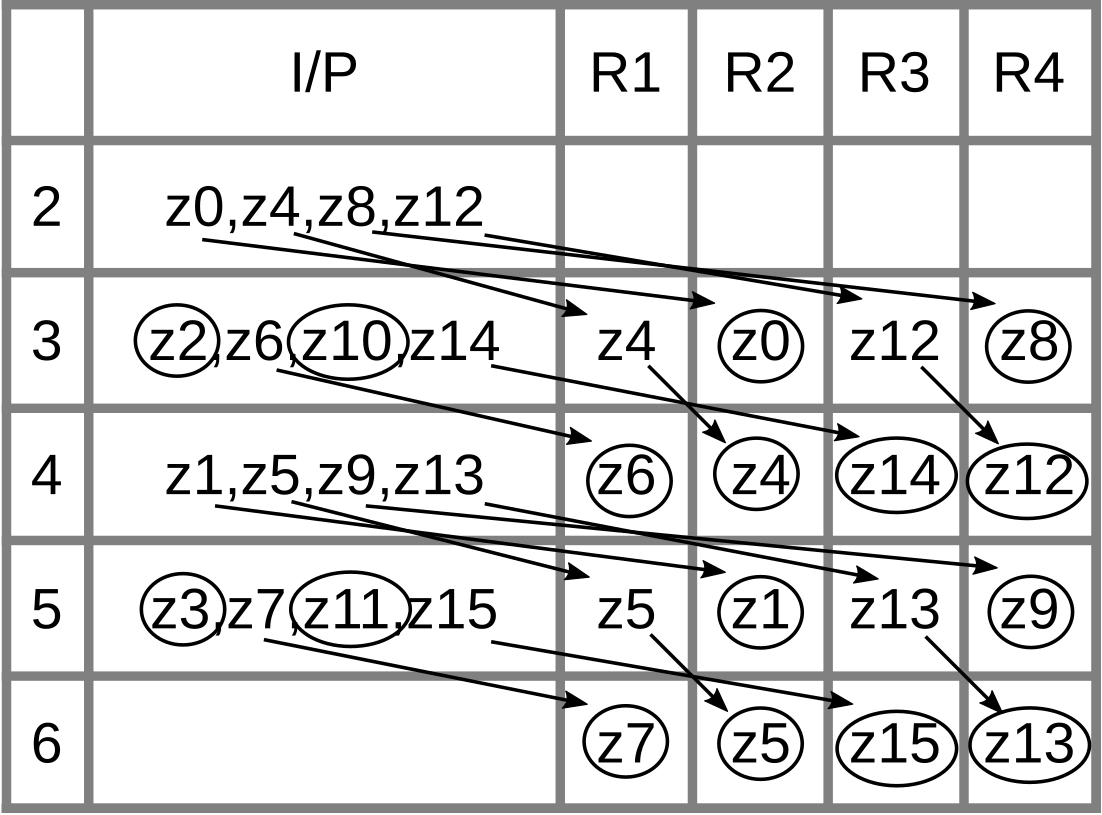
\includegraphics[height=0.25\paperheight]{./image/tab-life-b.png}
	    		\caption{\footnotesize Allocation table for stage 2.}
	    	\end{figure}
	    	\vspace{-0.75cm}
	    	\begin{figure}[h!] \centering
	    		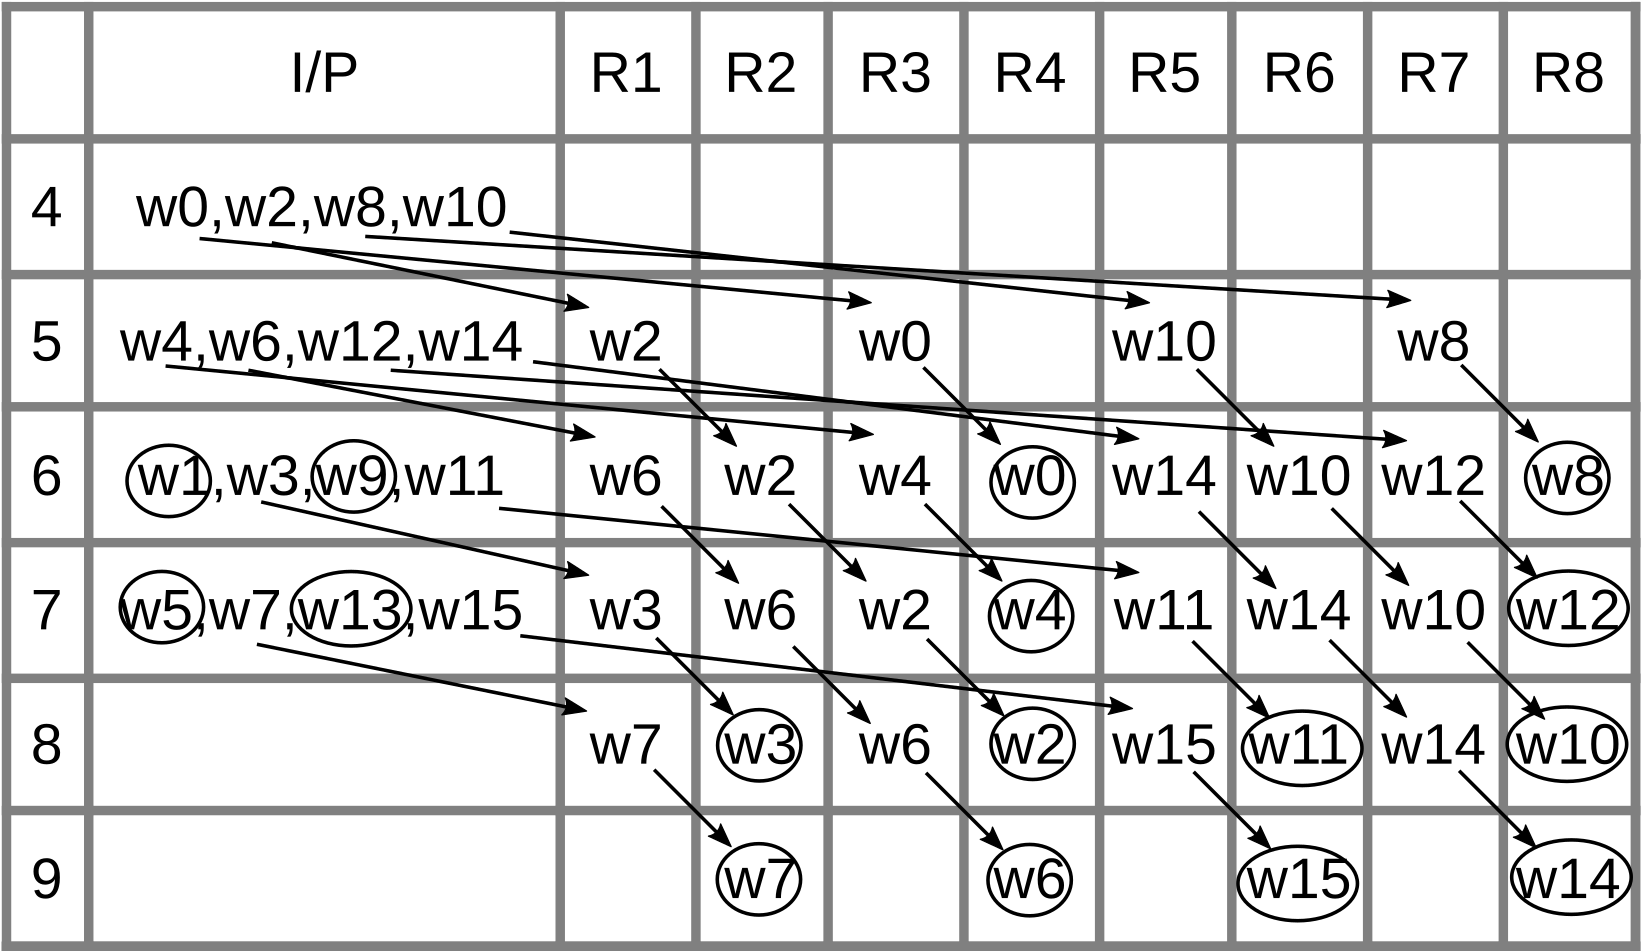
\includegraphics[height=0.30\paperheight]{./image/tab-life-c.png}
	    		\caption{\footnotesize Allocation table for stage 3.}
	    	\end{figure}  
   		\end{column}
	\end{columns}
\end{frame}

\begin{frame}
	\frametitle{\textbf{Design of FFT architecture via folding transformation}}
	\framesubtitle{\secname : \subsecname}
	\begin{block}{\centering \textbf{Folding architecture for radix-$2^3$ 16 points FFT}}
		\begin{itemize}\justifying\footnotesize
        	\item The values in the same column are data that flow in parallel and values in the same row flow through the same path in consecutive clock cycles. 
			\item For the rotator matrix, each number $k$ of the matrix represent a multiplication by $W^k_N$.
       	\end{itemize}
	\end{block}
		\vspace{-0.15cm}
		\begin{figure}[h!] \centering
		   	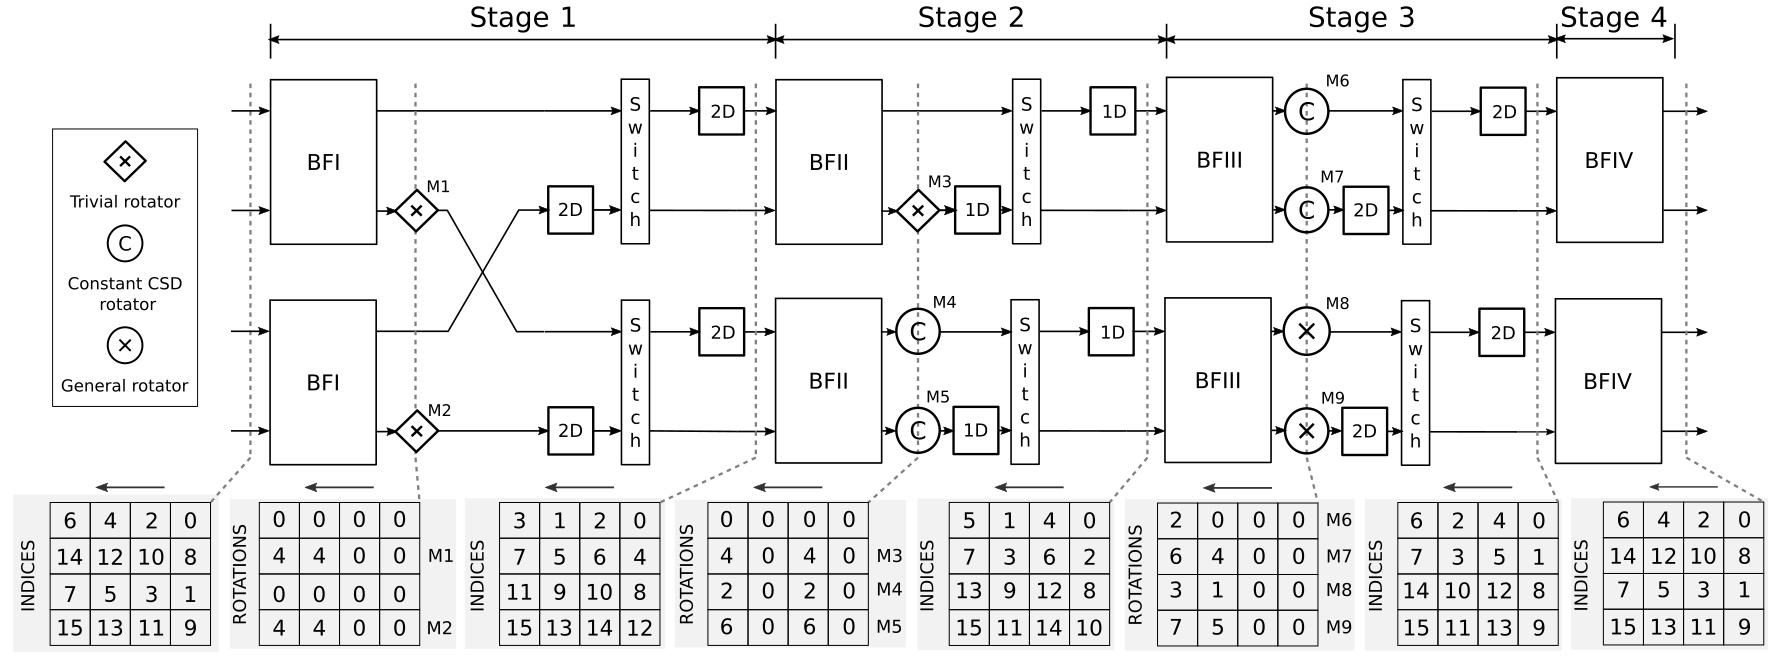
\includegraphics[width=0.875\paperwidth]{./image/folding-16.png}
		    \vspace{-0.15cm}
		    \caption{ \tiny Folding architecture for radix-$2^3$ 16 points FFT.}
		\end{figure}  
\end{frame}

\begin{frame}
	\frametitle{\textbf{Design of FFT architecture via folding transformation}}
	\framesubtitle{\secname : \subsecname}
	%\vspace{-0.5cm}
	\begin{block}{\centering }
	We can deduce the folding architecture for 128 points radix-$2^3$ following the same method. 
	\end{block}	
	\vspace{-0.15cm}
		\begin{figure}[h!] \centering
		   	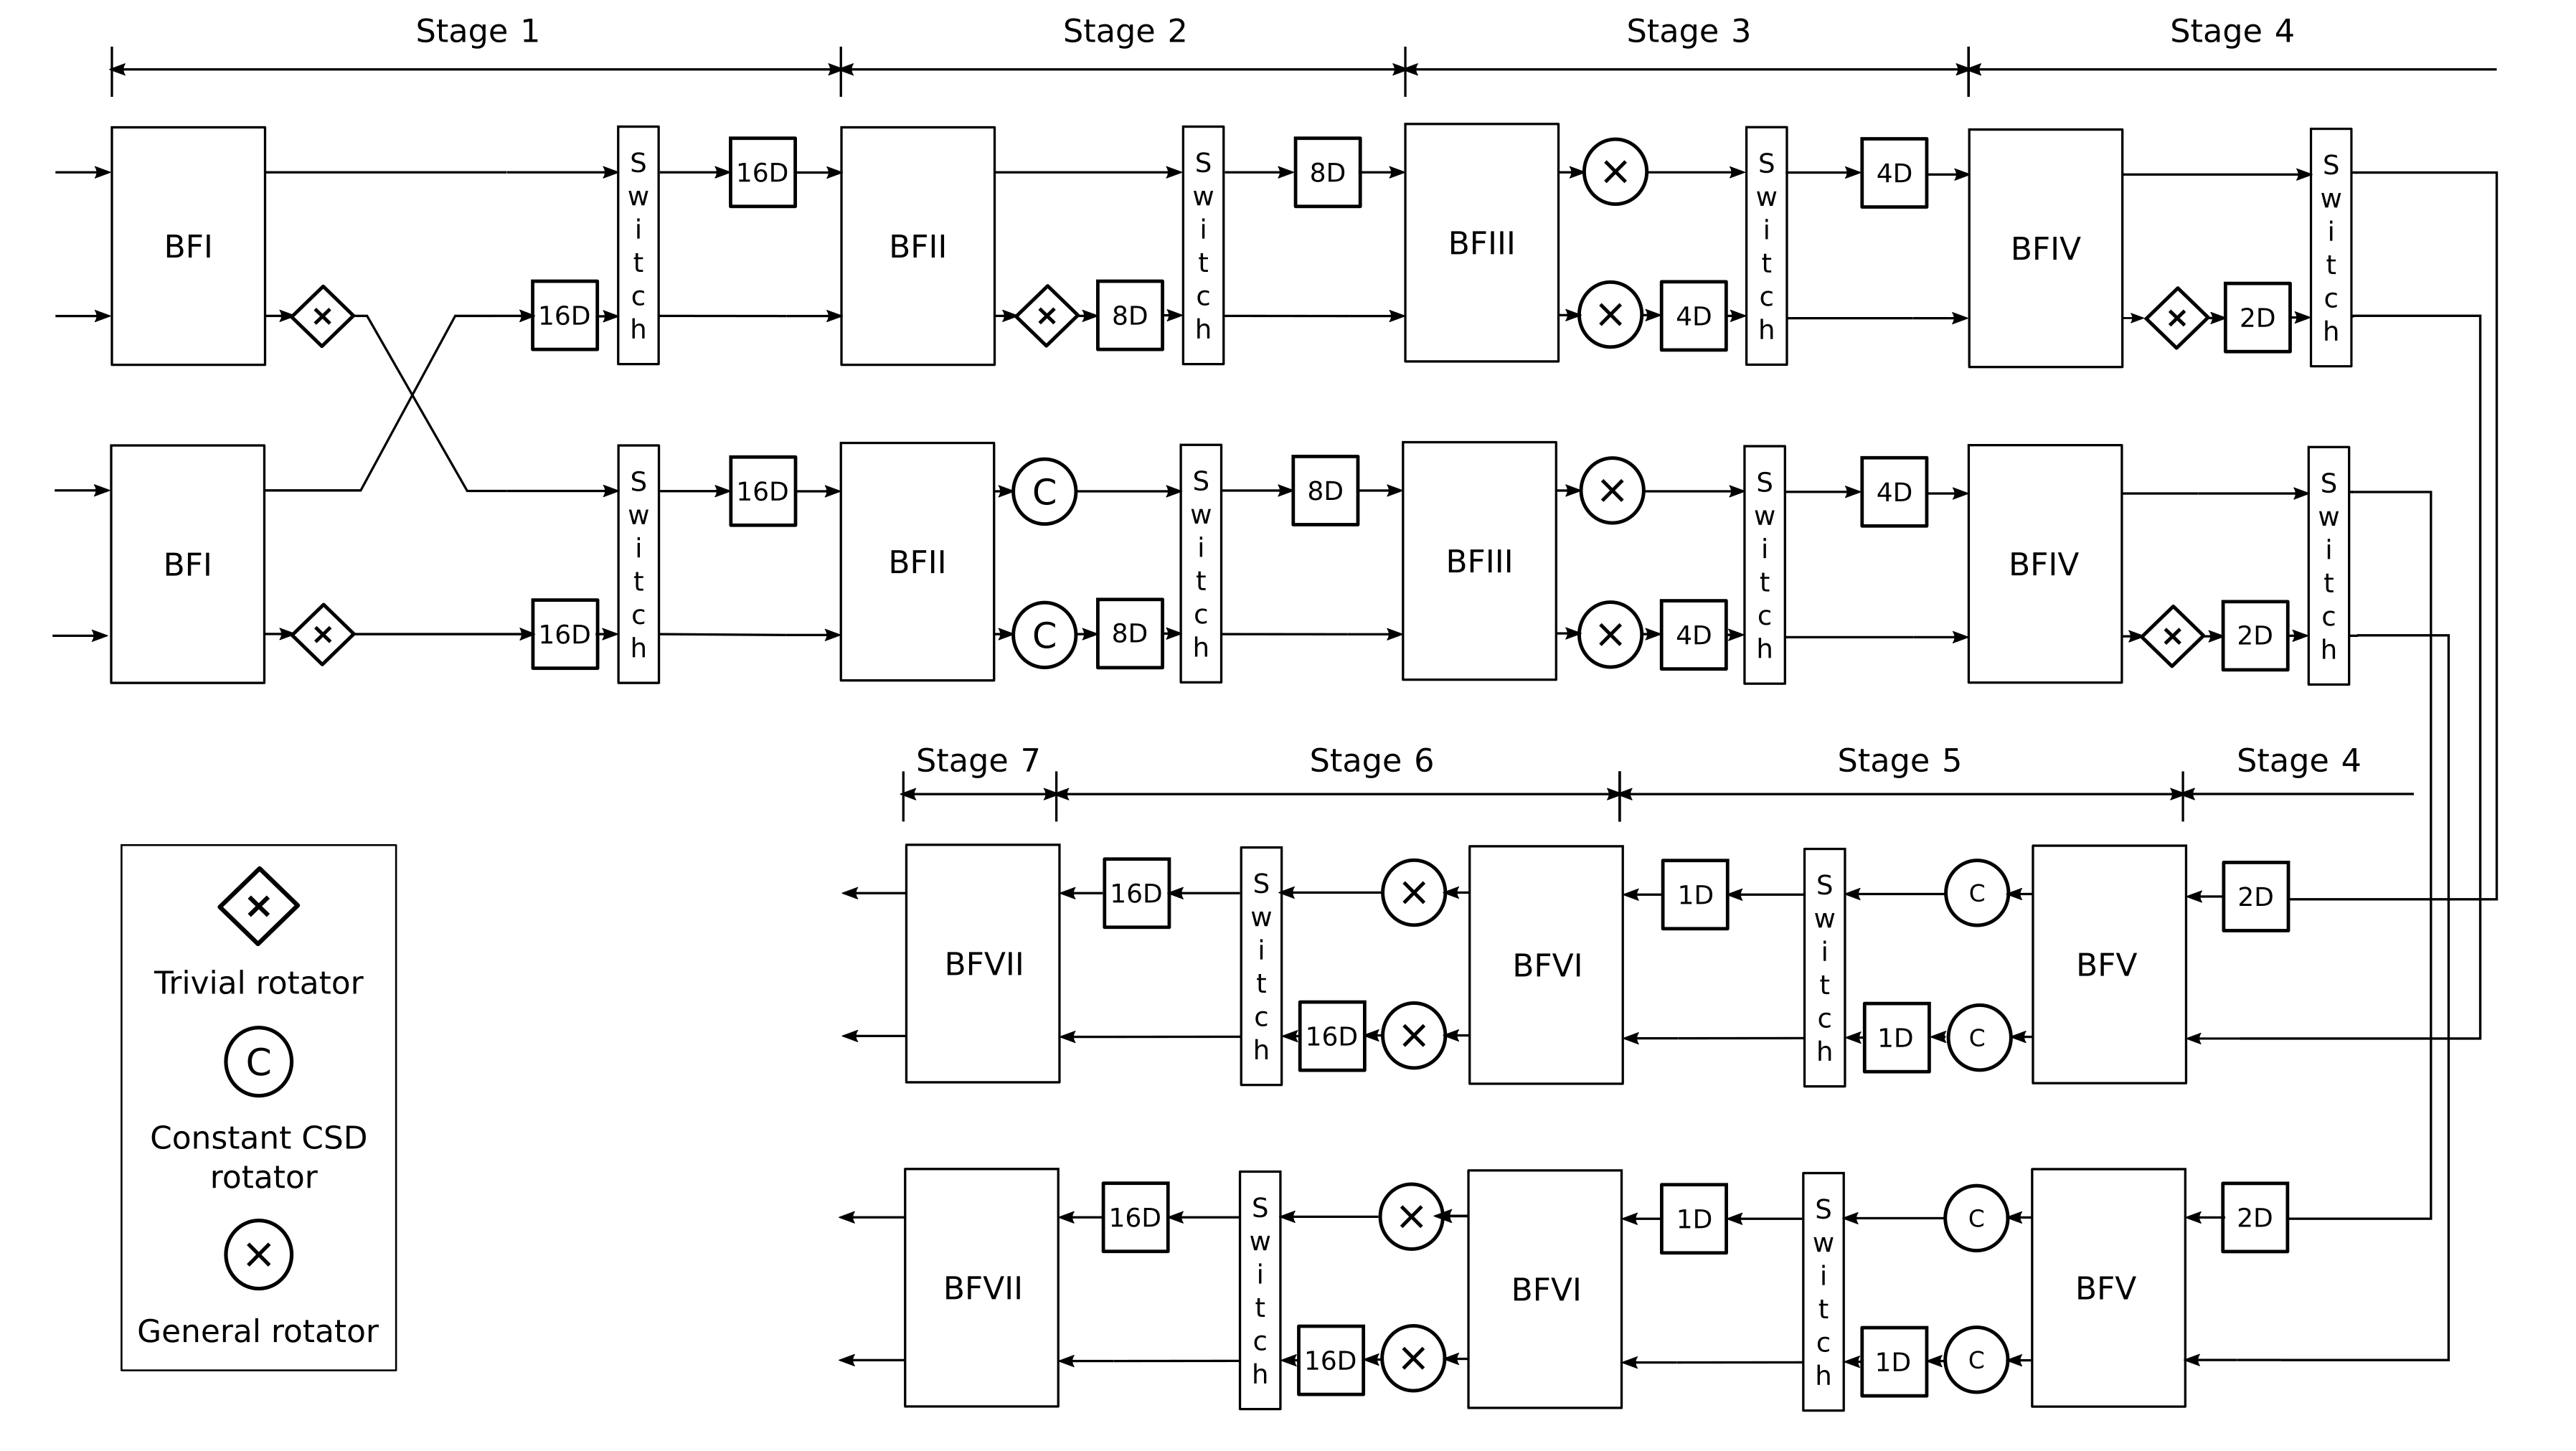
\includegraphics[width=0.75\paperwidth]{./image/folding-128.png}
		   	\vspace{-0.15cm}
		   	\caption{ \tiny Folding architecture for radix-$2^3$ 128 points FFT.}
		\end{figure}  	
\end{frame}